\documentclass{article}
\usepackage {inputenc, fullpage, listings, amsmath, graphicx, wasysym, comment}

\parindent 0pt

\title{%
   CSc 320: Foundations of Computer Science (Summer 2022)\\
    \Large Alex Holland\\
    Assignment 1\\
    }
\date{}

\begin{document}

\maketitle

{\bf Question 1}\\

\begin{center}
    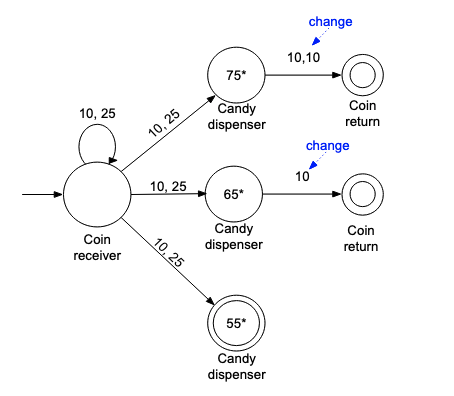
\includegraphics[width=0.7\textwidth]{1.png}
\end{center}
$*$ indicates the total coin amount ($\cent$) that the user has inputted into the candy machine.\\

\smallskip
{\bf Informal state diagram assumptions:}
\begin{itemize}
  \item The user does not input an amount that the machine cannot provide change for. E.g. the user cannot input $60^{\cent}$ because the machine can not give change in $5^{\cent}$ amounts.
  \item Only one candy can be bought and dispensed at a time.
  \item The user does not input excessive coin amounts that exceed the cost of the candy ($55^{\cent}$). E.g. the user wont input more then three $25^{\cent}$ coins because it is already enough to purchase a candy.
  \item $10,10$ indicates a change amount of $20^{\cent}$.
\end{itemize}

{\bf Question 2}\\
$L_A=\{w \in \Sigma^* | w$ contains the substring $bba\}$.\\
State diagram:\\
\begin{center}
    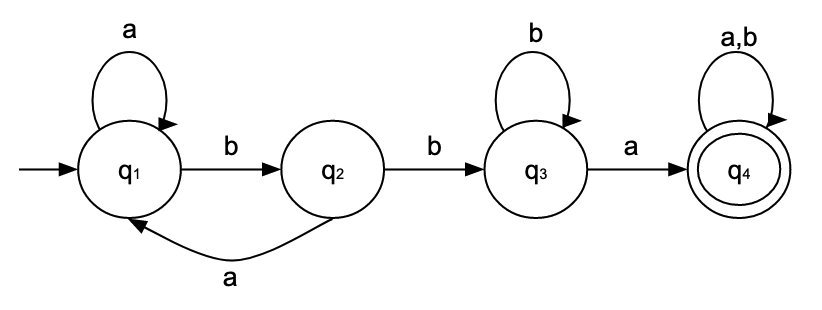
\includegraphics[width=0.6\textwidth]{2-1.png}
\end{center}

Transition Table:
\begin{center}
\begin{tabular}{||c c c||} 
 \hline
 $\delta$ & $a$ & $b$\\ [0.5ex] 
 \hline\hline
 $q_1$ & $q_1$ & $q_2$\\
 \hline
 $q_2$ & $q_1$ & $q_3$\\
 \hline
 $q_3$ & $q_4$ & $q_3$\\
 \hline
 $q_4$& $q_4$ & $q_4$\\
 \hline
\end{tabular}
\end{center}

\smallskip
$L_B=\{w \in \Sigma^* | w$ each pair of consecutive $bs$ in $w$ is separated by a substring of $as$ that is of length $3i,i>0\}$.\\

\begin{center}
    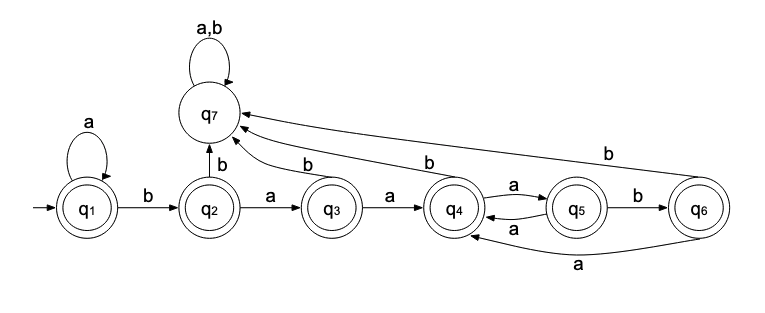
\includegraphics[width=1\textwidth]{2-2.png}
\end{center}

Transition Table:
\begin{center}
\begin{tabular}{||c c c||} 
 \hline
 $\delta$ & $a$ & $b$\\ [0.5ex] 
 \hline\hline
 $q_1$ & $q_1$ & $q_2$\\
 \hline
 $q_2$ & $q_3$ & $q_7$\\
 \hline
 $q_3$ & $q_4$ & $q_7$\\
 \hline
 $q_4$& $q_5$ & $q_7$\\
 \hline
 $q_5$& $q_4$ & $q_6$\\
 \hline
 $q_6$& $q_4$ & $q_7$\\
 \hline
 $q_7$& $q_7$ & $q_7$\\
 \hline
\end{tabular}
\end{center}

Assumptions:
\begin{itemize}
  \item "each pair of consecutive $bs$ in $w$ is separated by a substring of $as$" means that if we have 2 $bs$ next to each other as a pair, they will be separated by a substring of $3i, i > 0$ $as$. E.g. $baaab$ is an accepted string.
\end{itemize}

\bigskip
{\bf Question 3}\\
The state diagram $F1$ recognizes strings that have a maximum of one '1' symbol and unlimited '0' symbols. If more then one '1' symbol in the string $\omega$ is used in the $F1$, the input will become stuck in the transition state $C$.\\

Examples of strings $(\omega)$ accepted by $F1$:
\begin{equation*}
    \begin{split}
        0, \;1, \;01, \;10, \;00, \;100, \;010, \;001
    \end{split}
\end{equation*}
Examples of strings $(\omega)$ not accepted by $F1$:
\begin{equation*}
    \begin{split}
        11, \;110, \;011, \;101, \;111, \;1110, \;1101, \;0111
    \end{split}
\end{equation*}


{\bf Question 4}\\
$\omega_1=\epsilon$\\
The automation stays in $q1$ state (initial state), which is an accepted state. Hence, $\omega_1$ is accepted by $D$.\\

$\omega_2=0111$\\
\begin{equation*}
    \begin{split}
        \text{Start in } & q_1 \text{, read } 0\\
        \text{Start in } & q_3 \text{, read } 1\\
        \text{Start in } & q_4 \text{, read } 1\\
        \text{Start in } & q_3 \text{, read } 1\\
        \text{In } & q_4\\
    \end{split}
\end{equation*}
The string $\omega_2$ is accepted in $D$.\\

$\omega_3=100000100$\\
\begin{equation*}
    \begin{split}
        \text{Start in } & q_1 \text{, read } 1\\
        \text{Start in } & q_4 \text{, read } 0\\
        \text{Start in } & q_2 \text{, read } 0\\
        \text{Start in } & q_4 \text{, read } 0\\
        \text{Start in } & q_2 \text{, read } 0\\
        \text{Start in } & q_4 \text{, read } 0\\
        \text{Start in } & q_2 \text{, read } 1\\
        \text{Start in } & q_3 \text{, read } 0\\
        \text{Start in } & q_1 \text{, read } 0\\
        \text{In } & q_3\\
    \end{split}
\end{equation*}
The string $\omega_3$ is not accepted in $D$.\\

$\omega_4=1010110$\\
\begin{equation*}
    \begin{split}
        \text{Start in } & q_1 \text{, read } 1\\
        \text{Start in } & q_4 \text{, read } 0\\
        \text{Start in } & q_2 \text{, read } 1\\
        \text{Start in } & q_3 \text{, read } 0\\
        \text{Start in } & q_1 \text{, read } 1\\
        \text{Start in } & q_4 \text{, read } 1\\
        \text{Start in } & q_3 \text{, read } 0\\
        \text{In } & q_1\\
    \end{split}
\end{equation*}
The string $\omega_4$ is accepted in $D$.\\


$\omega_5=1111111$\\
\begin{equation*}
    \begin{split}
        \text{Start in } & q_1 \text{, read } 1\\
        \text{Start in } & q_4 \text{, read } 1\\
        \text{Start in } & q_3 \text{, read } 1\\
        \text{Start in } & q_4 \text{, read } 1\\
        \text{Start in } & q_3 \text{, read } 1\\
        \text{Start in } & q_4 \text{, read } 1\\
        \text{Start in } & q_3 \text{, read } 1\\
        \text{In } & q_4\\
    \end{split}
\end{equation*}
The string $\omega_5$ is accepted in $D$.\\

\break
{\bf Question 5}\\ 
$M=(\{p,q,r,s\},\{0,1\},\delta_{M},p,\{s\})$\\
\begin{center}
    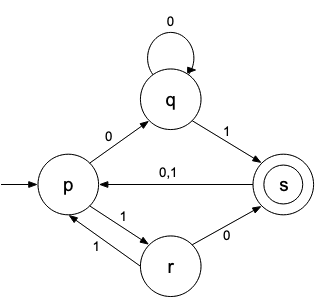
\includegraphics[width=0.35\textwidth]{5-1.png}
\end{center}

$N=(\{a,b\},\{0,1\},\delta_{N},a,\{a,b\})$\\
\begin{center}
    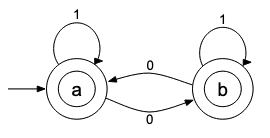
\includegraphics[width=0.31\textwidth]{5-2.png}
\end{center}


$A=(\{p,q,r,s,a,b\}, \Sigma, \delta, (p,a), \{(p,a),(q,a),(r,a),(s,a),(p,b),(q,b),(r,b)(s,b)\})$\\


Transition Table:
\begin{center}
\begin{tabular}{||c c c||} 
 \hline
 $\delta_{A}$ & 0 & 1\\ [0.5ex] 
 \hline\hline
 $(p,a)$ & $(q,b)$ & $(r,a)$\\
 \hline
 $(r,a)$ & $(s,b)$ & $(p,a)$\\
 \hline
 $(s,a)$ & $(p,b)$ & $(p,a)$\\
 \hline
 $(q,a)$ & $(q,b)$ & $(s,a)$\\
 \hline
 $(p,b)$ & $(q,a)$ & $(r,b)$\\
 \hline
 $(r,b)$ & $(s,a)$ & $(p,b)$\\
 \hline
 $(s,b)$ & $(p,a)$ & $(p,b)$\\
 \hline
 $(q,b)$ & $(q,a)$ & $(s,b)$\\
 \hline
\end{tabular}
\end{center}

Regular languages are closed under union, and since $N$ accepts all strings (all of it's states are accept states), determining $L(A) = L(M) \cup L(N)$ must mean that all states of $A$ are accept states.\\

\break
State Diagram:
\begin{center}
    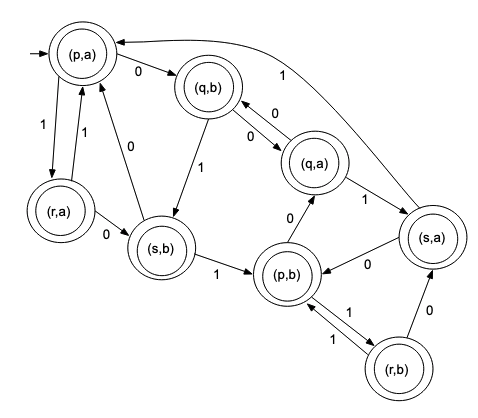
\includegraphics[width=0.6\textwidth]{5-3.png}
\end{center}


\end{document}
